% ============================================================
% REFERENCE TEMPLATE — exam-notes-generator-skill v1.1
% ============================================================
% PURPOSE: This file is the quality and formatting benchmark for all
% generated notes. The AI agent MUST open and read this file before
% generating any .tex output, and must match this structure exactly.
%
% NUMERICAL INVENTORY COMMENT BLOCK (place at top of every generated file):
% Module 1 — Type: [Name] ([N source] + [N constructed] = [total] total)
% Module 2 — Type: [Name] ([N source] + [N constructed] = [total] total)
% TOTAL: [X] original + [Y] constructed = [Z] worked examples
% NEW TIKZ DIAGRAMS: [N] ([list each diagram name and module])
%
% DIAGRAM EXTRACTION PIPELINE (run before writing any .tex):
% Step 1 — Extract embedded images from each source file:
%   PDF:  fitz.open(path) -> page.get_images(full=True) -> doc.extract_image(xref)
%         Also rasterize: page.get_pixmap(matrix=fitz.Matrix(2,2)) -> pix.save(png)
%   PPTX: Presentation(path) -> slide.shapes -> shape.image.blob  (shape_type==13)
%         Also soffice --headless --convert-to pdf -> then rasterize as above
%   DOCX: doc.part.rels.values() -> "image" in rel.reltype -> rel.target_part.blob
%
% Step 2 — Triage every image (log [KEEP] or [DISCARD] with reason):
%   KEEP:  Architecture/block diagrams, flowcharts, state machines, parse trees,
%          DP tables, plots, FST diagrams, comparison tables
%   DISCARD: University logos, slide chrome, decorative borders, exact duplicates
%
% Step 3 — OCR every KEEP image:
%   subprocess.run(["tesseract", img_path, "stdout"], capture_output=True, text=True)
%   Also visually inspect the image; write a caption sentence (what it shows +
%   what concept it illustrates + source file + slide/page number).
%
% Step 4 — Copy to /outputs/figures/diagrams/ with semantic name:
%   Format: m{N}_{topic_slug}.{ext}   e.g. m4_rnn_unrolled.png, m5_dfa_transition.png
%   Rules: no spaces, no generic names (image1.png is REJECTED), append _a/_b for variants
%
% Step 5 — Embed in .tex IMMEDIATELY after the paragraph that introduces the concept:
%   \begin{figure}[H]
%     \centering
%     \includegraphics[width=0.85\textwidth]{figures/diagrams/mN_topic_slug.png}
%     \caption{Full descriptive caption. Source: file.pptx, Slide N.}
%     \label{fig:mN_topic_slug}
%   \end{figure}
%   Width rules: \textwidth (wide/DP tables) | 0.85\textwidth (blocks/flowcharts) |
%                0.6\textwidth (tall trees) | 0.45\textwidth (small state machines)
%   NEVER use [h],[t],[b] — always [H] (float package)
%   NEVER place a diagram in a different \section than its theory
%
% Step 6 — When no extractable image exists for a concept but the source uses
%   a diagram, generate a TikZ diagram inline (see patterns below).
%   TikZ is always \begin{center}...\end{center} followed by \captionof{figure}{...}
% ============================================================

\documentclass[11pt,a4paper]{article}
\usepackage[utf8]{inputenc}
\usepackage[T1]{fontenc}
\usepackage{lmodern}
\usepackage{amsmath, amssymb, amsfonts}
\usepackage{graphicx}
\usepackage{booktabs}
\usepackage{geometry}
\usepackage{hyperref}
\usepackage{tcolorbox}
\usepackage{enumitem}
\usepackage{xcolor}
\usepackage{float}
\usepackage{longtable}
\usepackage{caption}
\usepackage{subcaption}
\usepackage{array}
\usepackage{multirow}
\usepackage{makecell}
\usepackage{colortbl}
\usepackage{tikz}
\usetikzlibrary{shapes,arrows,positioning,calc,decorations.pathreplacing,fit,backgrounds,matrix,shadows,trees}
\usepackage{pgfplots}
\pgfplotsset{compat=1.18}

\geometry{margin=0.9in}
\hypersetup{
    colorlinks=true,
    linkcolor=blue,
    filecolor=magenta,
    urlcolor=cyan,
    pdftitle={[Subject] Complete Study Material},
}

\setlist[itemize]{itemsep=0.5em, topsep=0.5em, parsep=0.2em}
\setlist[enumerate]{itemsep=0.5em, topsep=0.5em, parsep=0.2em}

% ============================================================
% TCOLORBOX LIBRARY SETUP (required for breakable boxes)
% ============================================================
\tcbuselibrary{skins,breakable}

% ============================================================
% NEWTCOLORBOX DEFINITIONS — STYLE INHERITANCE RULE
% ============================================================
% These are the CANONICAL box definitions for study notes.
% If a subject already has existing module .tex files, OPEN ONE,
% copy its \newtcolorbox definitions here verbatim, and delete
% these defaults. All modules of one subject must share the same
% box style for visual consistency.
%
% Pattern used in production (ML3, NLTP modules):

% Key concept / definition box (blue header)
\newtcolorbox{conceptbox}[1]{
    colback=blue!5!white, colframe=blue!60!black,
    fonttitle=\bfseries, title=#1,
    breakable, enhanced
}

% Worked numerical box — source example (blue)
\newtcolorbox{sourcebox}[1]{
    colback=blue!4!white, colframe=blue!70!black,
    fonttitle=\bfseries, title=\textbf{Worked Example #1},
    breakable, enhanced
}

% Worked numerical box — agent-constructed (green)
\newtcolorbox{constructedbox}[1]{
    colback=green!4!white, colframe=green!65!black,
    fonttitle=\bfseries, title=\textbf{Worked Example #1},
    breakable, enhanced
}

% Q&A box for solutions documents — question (gray)
\newtcolorbox{questionbox}{
    colback=gray!6, colframe=black!60,
    fonttitle=\bfseries, title=\textbf{Question},
    breakable, enhanced
}

% Q&A box for solutions documents — solution (blue)
\newtcolorbox{solutionbox}{
    colback=blue!4, colframe=blue!70,
    fonttitle=\bfseries, title=\textbf{Solution},
    breakable, enhanced
}

% Inline \qabox convenience alias (used in some subject styles)
% \newtcolorbox{qabox}[2]{colback=#1!5,colframe=#1!70,title=\textbf{#2},breakable,enhanced}

% ============================================================
% COMPILE INSTRUCTION (two-pass mandatory)
% ============================================================
% pdflatex -interaction=nonstopmode -output-directory <outdir> <file.tex>
% pdflatex -interaction=nonstopmode -output-directory <outdir> <file.tex>
% Check .log for "!" lines — zero is required before declaring completion.
% ============================================================

\title{\textbf{[Subject Name]\\Complete Study Material --- [Edition]}}
\author{Generated from course material with all numericals solved}
\date{}

\begin{document}

\maketitle
\tableofcontents
\newpage

% ============================================================
% MODULE 1 — THEORY SECTION WITH PROSE-FIRST STYLE
% ============================================================

\section{Module 1: [Module Name]}

\subsection{[Topic Name]}

% PROSE-FIRST RULE: ALWAYS open every \subsection and \subsubsection with
% 2-4 sentences of explanatory prose BEFORE any bullet list or enumeration.
% The paragraph must: (1) define the term, (2) explain its purpose,
% (3) state why it matters. Never start with \begin{itemize}.

\textbf{[Topic Name]} is [definition in one sentence]. Unlike [alternative approach],
it [distinguishing property], which makes it particularly useful for [application context].
This concept is foundational because [downstream significance in the subject].

The formal definition states that [formal statement]. In practice, [how it is computed
or applied]. For example, given [simple example], the result is [outcome], which
illustrates [key insight].

\begin{itemize}
    \item \textbf{Key Term A}: Complete-sentence definition. Explain not just what it is,
          but how it works and where it applies in this subject.
    \item \textbf{Key Term B}: Definition with elaboration connecting to Key Term A.
    \begin{itemize}
        \item Sub-point: preserve nested structure from source material exactly.
        \item Sub-point: do not flatten nested bullets into a single paragraph.
        \item Sub-point: each sub-bullet is a complete clause, not a fragment.
    \end{itemize}
    \item \textbf{Key Term C}: Definition with formula reference if applicable.
\end{itemize}

% ---- Key Concept tcolorbox (blue = key definition/principle from source) ----
\begin{tcolorbox}[colback=blue!5!white,colframe=blue!75!black,title=\textbf{Key Concept: [Name]}]
[State the principle in 1-2 sentences expanded from the source.] This matters because
[implication for exam or application]. The formal expression is:
\[
    \text{Formula} = \frac{\text{numerator}}{\text{denominator}}
\]
where [explain each symbol].
\end{tcolorbox}

% ============================================================
% TIKZ PATTERN 1: Architecture / Pipeline Block Diagram
% Use for: system architectures, pipelines, processing stages
% ============================================================
% If a diagram was extracted from the source, use \includegraphics instead:
% \begin{figure}[H]
%   \centering
%   \includegraphics[width=0.85\textwidth]{figures/diagrams/m1_topic_pipeline.png}
%   \caption{...full descriptive caption... (Source: file.pptx, Slide N)}
%   \label{fig:m1_topic_pipeline}
% \end{figure}
%
% Use TikZ only when no extractable image exists for the concept:

\begin{center}
\begin{tikzpicture}[
    node distance=1.5cm,
    box/.style={rectangle, draw, rounded corners, minimum width=2.8cm,
                minimum height=1cm, align=center, thick, fill=blue!10},
    data/.style={rectangle, draw, dashed, rounded corners, minimum width=2.5cm,
                 minimum height=0.8cm, align=center, fill=gray!10},
    arrow/.style={->, >=stealth, thick}
]
\node[data] (input) at (0,0) {\textbf{Input}\\[raw data]};
\node[box] (step1) at (4,0) {\textbf{Step 1}\\[processing]};
\node[box] (step2) at (8,0) {\textbf{Step 2}\\[transformation]};
\node[box, fill=green!15] (output) at (12,0) {\textbf{Output}\\[result]};

\draw[arrow] (input) -- (step1);
\draw[arrow] (step1) -- (step2);
\draw[arrow] (step2) -- (output);

\node[font=\scriptsize, above] at (2, 0.3) {[label]};
\node[font=\scriptsize, above] at (6, 0.3) {[label]};
\node[font=\scriptsize, above] at (10, 0.3) {[label]};
\end{tikzpicture}
\end{center}
\captionof{figure}{[Descriptive caption: what this pipeline shows, what concept it
illustrates, which source file and slide it came from. E.g.: ``Naive Bayes classification
pipeline showing document tokenization, prior and likelihood estimation, and posterior
maximization. (Source: Module3-NB.pptx, Slide 8)'']}

% ============================================================
% TIKZ PATTERN 2: Algorithm Flowchart (decision diamond)
% Use for: iterative algorithms, decision procedures, control flow
% ============================================================

\begin{center}
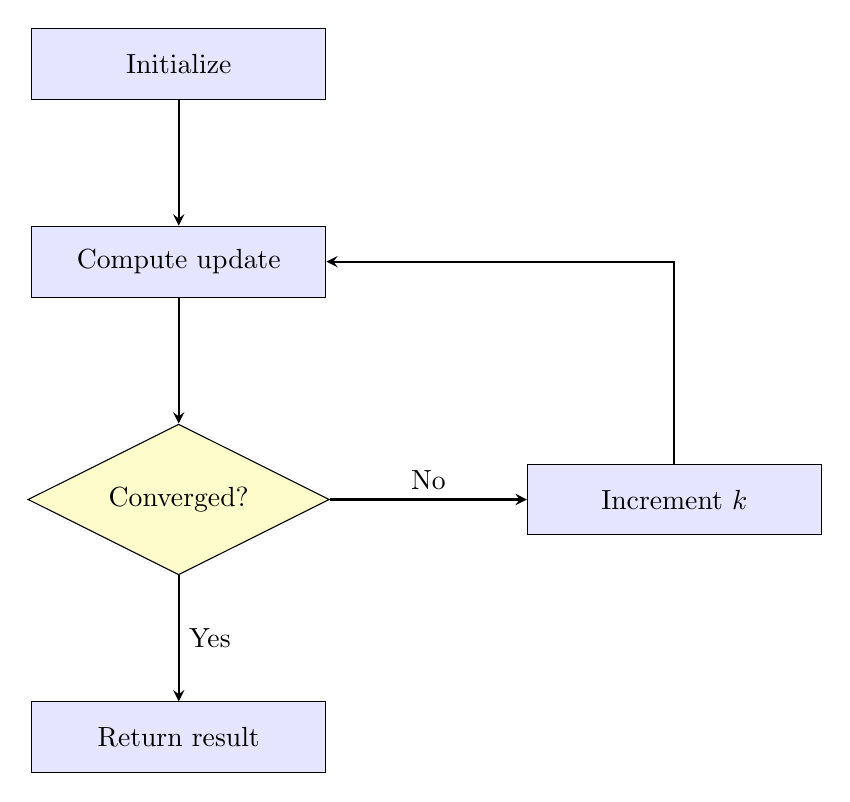
\begin{tikzpicture}[
    node distance=1.6cm,
    box/.style={rectangle, draw, fill=blue!10, text width=3.5cm,
                minimum height=0.9cm, align=center},
    decision/.style={diamond, draw, fill=yellow!20, text width=2.5cm,
                     minimum height=0.9cm, align=center, aspect=2},
    arrow/.style={->, >=stealth, thick}
]
\node[box] (init) {Initialize};
\node[box, below=of init] (step) {Compute update};
\node[decision, below=of step] (check) {Converged?};
\node[box, below=of check] (done) {Return result};
\node[box, right=2.5cm of check] (loop) {Increment $k$};

\draw[arrow] (init) -- (step);
\draw[arrow] (step) -- (check);
\draw[arrow] (check) -- node[right] {Yes} (done);
\draw[arrow] (check) -- node[above] {No} (loop);
\draw[arrow] (loop) |- (step);
\end{tikzpicture}
\end{center}
\captionof{figure}{[Algorithm name] iteration loop. [Explain what triggers convergence
and what the output represents. Source: file.pptx, Slide N.]}

% ============================================================
% TIKZ PATTERN 3: Tree (parse tree, probability tree, hierarchy)
% Use for: parse trees, decision trees, chain rule probability trees
% ============================================================

\begin{center}
\begin{tikzpicture}[
    level 1/.style={sibling distance=4cm, level distance=1.5cm},
    level 2/.style={sibling distance=2cm, level distance=1.5cm},
    level 3/.style={sibling distance=1cm, level distance=1.2cm},
    every node/.style={font=\small}
]
\node {S}
    child { node {NP}
        child { node {Det} child { node {the} } }
        child { node {N}   child { node {cat} } }
    }
    child { node {VP}
        child { node {V}   child { node {sat} } }
        child { node {PP}
            child { node {P}  child { node {on} } }
            child { node {NP} child { node {mat} } }
        }
    };
\end{tikzpicture}
\end{center}
\captionof{figure}{Parse tree for ``the cat sat on the mat'' showing hierarchical
constituent structure with NP and VP phrases. (Source: [file.pptx, Slide N])}

% ============================================================
% TIKZ PATTERN 4: DFA / State Machine
% Use for: automata, finite state machines, HMM state transitions
% ============================================================

\begin{center}
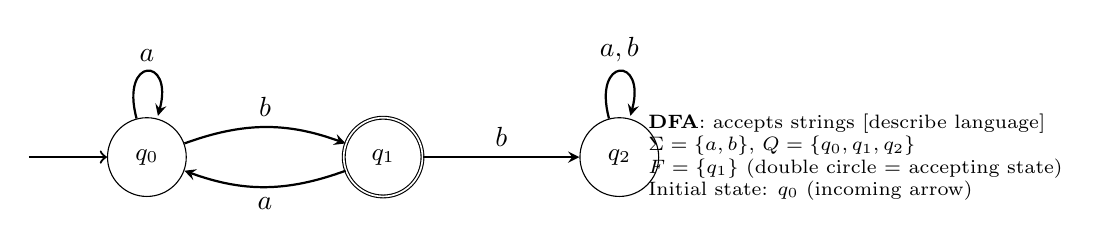
\begin{tikzpicture}[
    node distance=3cm,
    state/.style={circle, draw, minimum size=1cm, font=\small},
    finalstate/.style={circle, draw, minimum size=1cm, font=\small, double},
    arrow/.style={->, >=stealth, thick}
]
\node[state] (q0) at (0,0) {$q_0$};
\draw[->, thick] (-1.5, 0) -- (q0);   % initial arrow
\node[finalstate] (q1) at (3,0) {$q_1$};
\node[state] (q2) at (6,0) {$q_2$};

\draw[arrow] (q0) edge[loop above] node[above] {$a$} (q0);
\draw[arrow] (q0) edge[bend left=20] node[above] {$b$} (q1);
\draw[arrow] (q1) edge[bend left=20] node[below] {$a$} (q0);
\draw[arrow] (q1) -- node[above] {$b$} (q2);
\draw[arrow] (q2) edge[loop above] node[above] {$a,b$} (q2);

\node[align=left, font=\scriptsize] at (9, 0) {
\textbf{DFA}: accepts strings [describe language]\\
$\Sigma = \{a, b\}$, $Q = \{q_0, q_1, q_2\}$\\
$F = \{q_1\}$ (double circle = accepting state)\\
Initial state: $q_0$ (incoming arrow)
};
\end{tikzpicture}
\end{center}
\captionof{figure}{DFA state transition diagram for [language description]. Double circle
denotes accepting state(s); incoming unlabelled arrow marks the initial state.
(Source: [file.pptx, Slide N])}

% ============================================================
% TIKZ PATTERN 5: FST (Finite State Transducer)
% Use for: morphological parsing, string transduction
% ============================================================

\begin{center}
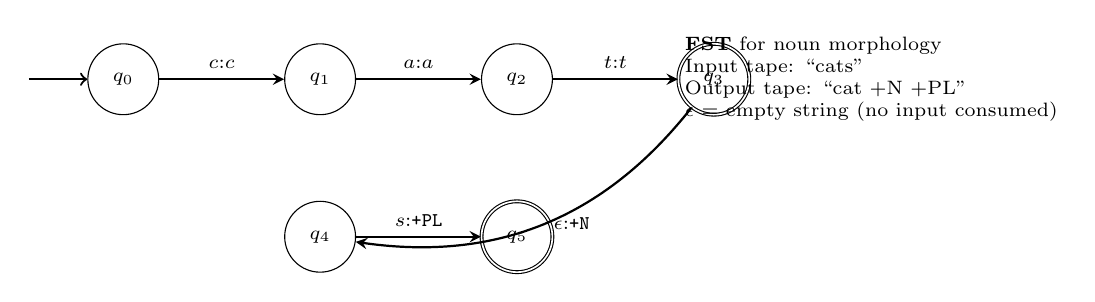
\begin{tikzpicture}[
    node distance=2.5cm,
    fststate/.style={circle, draw, minimum size=0.9cm, font=\scriptsize},
    fstfinal/.style={circle, draw, minimum size=0.9cm, font=\scriptsize, double},
    arrow/.style={->, >=stealth, thick}
]
\node[fststate] (q0) at (0,0) {$q_0$};
\draw[->, thick] (-1.2, 0) -- (q0);
\node[fststate] (q1) at (2.5,0) {$q_1$};
\node[fststate] (q2) at (5,0) {$q_2$};
\node[fstfinal] (q3) at (7.5,0) {$q_3$};

\draw[arrow] (q0) -- node[above, font=\scriptsize] {$c$:$c$} (q1);
\draw[arrow] (q1) -- node[above, font=\scriptsize] {$a$:$a$} (q2);
\draw[arrow] (q2) -- node[above, font=\scriptsize] {$t$:$t$} (q3);

\node[fststate] (q4) at (2.5,-2) {$q_4$};
\node[fstfinal] (q5) at (5,-2) {$q_5$};
\draw[arrow] (q3) edge[bend left=30] node[right, font=\scriptsize] {$\epsilon$:\texttt{+N}} (q4);
\draw[arrow] (q4) -- node[above, font=\scriptsize] {$s$:\texttt{+PL}} (q5);

\node[font=\scriptsize, align=left] at (9.5, 0) {
\textbf{FST} for noun morphology\\
Input tape: ``cats''\\
Output tape: ``cat +N +PL''\\
$\epsilon$ = empty string (no input consumed)
};
\end{tikzpicture}
\end{center}
\captionof{figure}{Finite State Transducer (FST) for English noun morphology. Reads the
surface form ``cats'' from the input tape and writes the lexical form ``cat +N +PL'' on
the output tape. (Source: [file.pptx, Slide N])}

% ============================================================
% TIKZ PATTERN 6: Unrolled sequence / shared-weight diagram
% Use for: RNNs, HMMs, sequential models
% ============================================================

\begin{center}
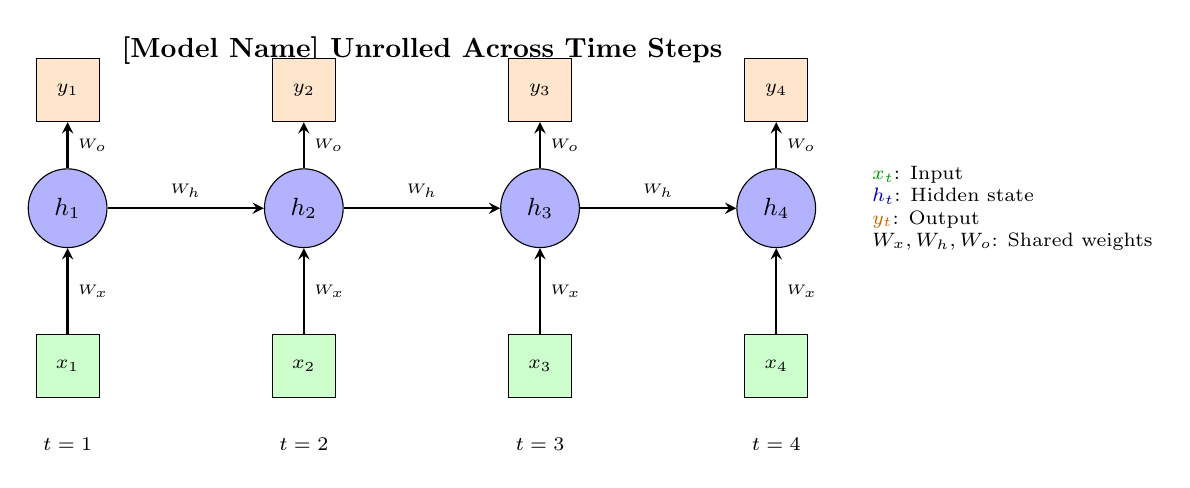
\begin{tikzpicture}[
    input/.style={rectangle, draw, fill=green!20, minimum size=0.8cm, font=\scriptsize},
    hidden/.style={circle, draw, fill=blue!30, minimum size=1cm, font=\small\bfseries},
    output/.style={rectangle, draw, fill=orange!20, minimum size=0.8cm, font=\scriptsize},
    arrow/.style={->, >=stealth, thick}
]
\node[font=\bfseries] at (4.5, 3) {[Model Name] Unrolled Across Time Steps};

\foreach \t/\x in {1/0, 2/3, 3/6, 4/9} {
    \node[hidden] (h\t) at (\x, 1) {$h_{\t}$};
    \node[input]  (x\t) at (\x,-1) {$x_{\t}$};
    \node[output] (y\t) at (\x, 2.5) {$y_{\t}$};
    \draw[arrow] (x\t) -- (h\t) node[midway, right, font=\tiny] {$W_x$};
    \draw[arrow] (h\t) -- (y\t) node[midway, right, font=\tiny] {$W_o$};
    \node[font=\scriptsize] at (\x,-2) {$t=\t$};
}
\draw[arrow] (h1) -- (h2) node[midway, above, font=\tiny] {$W_h$};
\draw[arrow] (h2) -- (h3) node[midway, above, font=\tiny] {$W_h$};
\draw[arrow] (h3) -- (h4) node[midway, above, font=\tiny] {$W_h$};

\node[align=left, font=\scriptsize] at (12, 1) {
\textcolor{green!60!black}{$x_t$}: Input\\
\textcolor{blue!70!black}{$h_t$}: Hidden state\\
\textcolor{orange!80!black}{$y_t$}: Output\\
$W_x, W_h, W_o$: Shared weights
};
\end{tikzpicture}
\end{center}
\captionof{figure}{[Model name] unrolled over 4 time steps, showing weight sharing
($W_x$, $W_h$, $W_o$ are identical at every step) and how the hidden state $h_t$
carries information forward. (Source: [file.pptx, Slide N])}

% ============================================================
% TIKZ PATTERN 7: pgfplots bar chart
% Use for: comparison of metrics, perplexity/accuracy across models
% ============================================================

\begin{center}
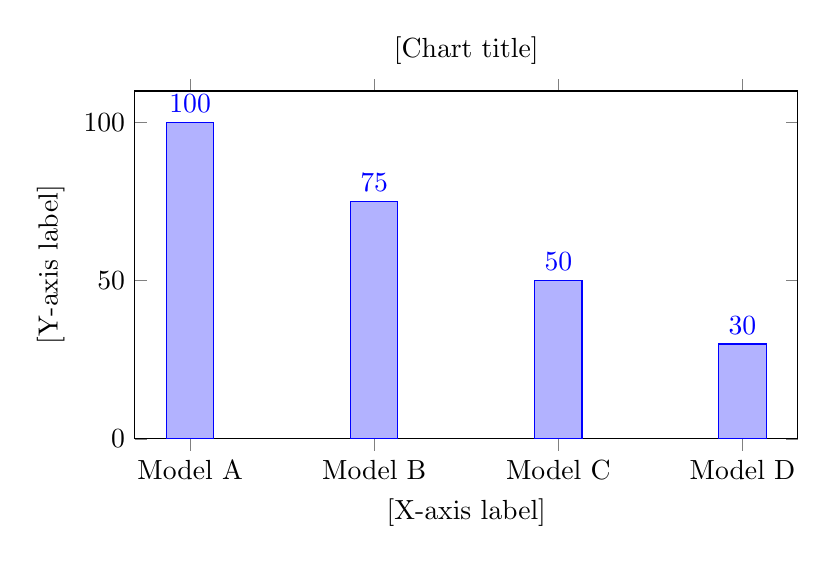
\begin{tikzpicture}
\begin{axis}[
    width=10cm, height=6cm,
    ybar,
    symbolic x coords={Model A, Model B, Model C, Model D},
    xtick=data,
    xlabel={[X-axis label]},
    ylabel={[Y-axis label]},
    ymin=0,
    bar width=0.6cm,
    nodes near coords,
    title={[Chart title]},
]
\addplot coordinates {(Model A, 100) (Model B, 75) (Model C, 50) (Model D, 30)};
\end{axis}
\end{tikzpicture}
\end{center}
\captionof{figure}{[Metric] comparison across [models/conditions]. Lower/higher values
indicate [interpretation]. (Source: [file.pptx, Slide N])}

% ============================================================
% WORKED EXAMPLES — THREE TCOLORBOX COLOURS
% ============================================================
%
% COLOUR CONVENTION (mandatory):
%   blue  (colback=blue!5!white,  colframe=blue!75!black)  → reproduced from source
%   green (colback=green!5!white, colframe=green!75!black) → agent-constructed extra
%   yellow(colback=yellow!5!white,colframe=yellow!75!black)→ theoretical analysis /
%                                                            numerical insight box
%
% NUMBERING: global sequential "Worked Example N" — never reset between sections.
% PLACEMENT: immediately after the \subsection that introduces the method. Never at end.
% MINIMUM: 3 total per numerical type (1 source + 2 constructed, or 0 source + 2 constructed).

\begin{tcolorbox}[colback=blue!5!white,colframe=blue!75!black,
    title=\textbf{Worked Example 1: [Title] (from source)}]

\textbf{Given}: [All input values, model parameters, or problem setup exactly as in source]

\textbf{Find}: [What the student must calculate or determine]

\textbf{Solution}:
\begin{enumerate}
    \item \textbf{[Step label]}: [Full explanation of computation, including formula used
          and intermediate result. Show all arithmetic.]
    \[
        \text{formula} = \frac{a}{b} = \text{value}
    \]
    \item \textbf{[Step label]}: [Next computation.]
    \[
        \text{formula} = \text{result}
    \]
    \item \textbf{[Step label]}: [Final computation.]
\end{enumerate}

\textbf{Answer}: [Final numeric or symbolic result, bolded if scalar]

\textbf{Interpretation}: [One sentence: what this result means in the context of the topic.]
\end{tcolorbox}

\begin{tcolorbox}[colback=green!5!white,colframe=green!75!black,
    title=\textbf{Worked Example 2: [Title] (constructed — different inputs, same method)}]

\textbf{Given}: [Inputs chosen to illustrate a different case or edge condition]

\textbf{Find}: [Same type of question as Example 1]

\textbf{Solution}:
\begin{enumerate}
    \item \textbf{[Step label]}: [Computation with formula.]
    \[
        \text{formula} = \text{value}
    \]
    \item \textbf{[Step label]}: [Result.]
\end{enumerate}

\textbf{Answer}: [Result]

\textbf{Interpretation}: [Why this case is instructive — e.g. zero probability, boundary, etc.]
\end{tcolorbox}

\begin{tcolorbox}[colback=green!5!white,colframe=green!75!black,
    title=\textbf{Worked Example 3: [Edge Case Title] (constructed)}]

\textbf{Given}: [Inputs for edge case — unseen word, empty set, boundary value, etc.]

\textbf{Find}: [Question]

\textbf{Solution}:
\begin{enumerate}
    \item \textbf{[Step label]}: [Edge case handling — explain what changes vs. normal case.]
    \item \textbf{[Step label]}: [Result.]
\end{enumerate}

\textbf{Answer}: [Result]

\textbf{Interpretation}: [Why this edge case appears in exams / what it tests.]
\end{tcolorbox}

% Yellow box: use for theoretical insights, analysis, or key derivation steps
\begin{tcolorbox}[colback=yellow!5!white,colframe=yellow!75!black,
    title=\textbf{Theoretical Analysis: [Topic]}]
[Expand on the mathematical relationship or conceptual insight. Derive or explain
a formula result. This box is for analysis, not a worked problem with specific inputs.]
\[
    \text{key equation or derivation step}
\]
[Continue explanation. Connect to the worked examples above.]
\end{tcolorbox}

% ============================================================
% ALGORITHM TRACE WITH DP TABLE
% Use for: Viterbi, CKY, Edit Distance, any tabular dynamic programming
% ============================================================

\begin{tcolorbox}[colback=blue!5!white,colframe=blue!75!black,
    title=\textbf{Worked Example 4: [Algorithm] Trace (from source)}]

\textbf{Given}: Input = [sequence/string/values], model = [parameters]

\textbf{Find}: Trace the algorithm step by step. Fill the DP table.

\textbf{Solution} --- DP table:

\begin{center}
\begin{tabular}{|c|c|c|c|c|}
\hline
 & \textbf{Col 1} & \textbf{Col 2} & \textbf{Col 3} & \textbf{Col 4} \\ \hline
\textbf{Row A} & [val] & [val] & [val] & [val] \\ \hline
\textbf{Row B} & [val] & [val] & [val] & [val] \\ \hline
\textbf{Row C} & [val] & [val] & [val] & [val] \\ \hline
\end{tabular}
\end{center}

\begin{enumerate}
    \item \textbf{Initialization}: [How row/column 0 is filled and why.]
    \item \textbf{Fill}: [Recurrence relation with formula:] $dp[i][j] = \min/\max(...)$
    \item \textbf{Backtrack}: [How to read the solution from the table.]
\end{enumerate}

\textbf{Answer}: [Final value from table, with backtracked path if applicable]

\textbf{Interpretation}: [What this result means — cost, probability, parse, etc.]
\end{tcolorbox}

% ============================================================
% MISSING COVERAGE (mandatory section if any syllabus gaps exist)
% ============================================================

\section*{Missing Coverage}

The following syllabus topics had no matching source material in the provided files.
Content was not invented --- these gaps are reported for the student's awareness:

\begin{itemize}
    \item \textbf{[Topic X]}: No slides, PDF pages, or textbook sections covered this topic
          in the provided source set.
    \item \textbf{[Topic Y]}: Mentioned in syllabus but not elaborated in any provided file.
\end{itemize}

% ============================================================
% SOLUTIONS DOCUMENT PATTERN
% ============================================================
% Use this pattern when the request is for solutions to practice questions
% (triggered by: "solutions", "solve", "answers to practice questions").
%
% Output file: <subject-slug>-practice-questions-solutions.tex
% One question+solution pair per \subsection*{Q N.M Title}
%
% RULES FOR SOLUTION BOXES:
%   1. ALWAYS open with a conceptual paragraph (2-4 sentences) explaining the theory.
%      Never start a solution box with a bare bullet list or fragment.
%   2. Use \textbf{label:} sub-sections within the solution for multi-part questions.
%   3. Show every arithmetic step for numerical sub-questions.
%   4. End numerical solutions with \boxed{answer} and an interpretation sentence.
%   5. Solutions should be EXPLANATORY, not just a list of facts.

% ---- Example question/solution pair ----

% \subsection*{Q1.1 [Question Title]}
% \begin{tcolorbox}[colback=gray!6,colframe=black!60,breakable,title=\textbf{Question}]
% [Question text verbatim from the source file]
% \end{tcolorbox}
% \begin{tcolorbox}[colback=blue!4,colframe=blue!70,breakable,title=\textbf{Solution}]
%
% \textbf{[Concept Name] --- Background:}
%
% [2-4 sentence conceptual paragraph. Define the concept, explain its purpose,
% state why it matters. This paragraph must make the solution self-contained.]
%
% \textbf{[Sub-question or part label]:}
% \begin{itemize}
%   \item \textbf{Key element}: [Explanation with 1-2 sentences, not a fragment]
%   \item \textbf{Key element}: [Explanation]
% \end{itemize}
%
% \textbf{Numerical calculation (if applicable):}
% \[
%   \text{formula} = \text{value}
% \]
% [Explain what the number means in context.]
%
% \textbf{Conclusion:} [1 sentence summarising the answer.]
% \end{tcolorbox}

% ============================================================
% END OF REFERENCE TEMPLATE
% ============================================================
% To use: copy this file, replace all [bracketed placeholders],
% fill in actual content, run two-pass pdflatex, verify zero ! lines.
% ============================================================

\end{document}